\documentclass[conference]{IEEEtran}
\usepackage[top=3cm, bottom=2cm, left=2cm, right=2cm, columnsep=20pt]{geometry}
\usepackage{pdfpages}
\usepackage{graphicx}
\usepackage{etoolbox}
\apptocmd{\sloppy}{\hbadness 10000\relax}{}{}
% \usepackage[numbers]{natbib}
\usepackage[T1]{fontenc}
\usepackage{ragged2e}
\usepackage[french]{babel}
\usepackage{listings}
\usepackage{color}
\usepackage{soul}
\usepackage[utf8]{inputenc}
\usepackage[export]{adjustbox}
\usepackage{caption}
\usepackage{amsmath}
\usepackage{amssymb}
\usepackage{float}
\usepackage{csquotes}
\usepackage{fancyhdr}
\usepackage{wallpaper}
\usepackage{siunitx}
\usepackage[indent]{parskip}
\usepackage{textcomp}
\usepackage{gensymb}
\usepackage{multirow}
\usepackage[hidelinks]{hyperref}
\usepackage{abstract}
\usepackage{subcaption}
\usepackage{tabularx}

% \renewcommand{\abstractnamefont}{\normalfont\bfseries}
% \renewcommand{\abstracttextfont}{\normalfont\itshape}
\usepackage{titlesec}
% \titleformat{\section}{\large\bfseries}{\thesection}{1em}{}
% \titleformat{\subsection}{\normalsize\bfseries}{\thesubsection}{1em}{}
% \titleformat{\subsubsection}{\normalsize\bfseries}{\thesubsubsection}{1em}{}

\usepackage{xcolor}
\definecolor{codegreen}{rgb}{0,0.6,0}
\definecolor{codegray}{rgb}{0.5,0.5,0.5}
\definecolor{codepurple}{rgb}{0.58,0,0.82}
\definecolor{backcolour}{rgb}{0.95,0.95,0.92}
\lstdefinestyle{mystyle}{
    backgroundcolor=\color{backcolour},   
    commentstyle=\color{codegreen},
    keywordstyle=\color{magenta},
    numberstyle=\tiny\color{codegray},
    stringstyle=\color{codepurple},
    basicstyle=\ttfamily\footnotesize,
    breakatwhitespace=false,         
    breaklines=true,                 
    captionpos=b,                    
    keepspaces=true,                 
    numbers=left,                    
    numbersep=5pt,                  
    showspaces=false,                
    showstringspaces=false,
    showtabs=false,                  
    tabsize=2
}
\lstset{style=mystyle}

\usepackage[most]{tcolorbox}
\newtcolorbox{note}[1][]{
  enhanced jigsaw,
  borderline west={2pt}{0pt}{black},
  sharp corners,
  boxrule=0pt, 
  fonttitle={\large\bfseries},
  coltitle={black},
  title={Note:\ },
  attach title to upper,
  #1
}

%----------------------------------------------------

\setlength{\parindent}{0pt}
\DeclareCaptionLabelFormat{mycaptionlabel}{#1 #2}
\captionsetup[figure]{labelsep=colon}
\captionsetup{labelformat=mycaptionlabel}
\captionsetup[figure]{name={Figure }}
\captionsetup[table]{name=Tableau}
\newcolumntype{Y}[1]{>{\Centering\hspace{0pt}\hsize=#1\hsize}X}
\newcommand{\inlinecode}{\normalfont\texttt}
\usepackage{enumitem}
\setlist[itemize]{label=\textbullet}

\begin{document}

%----------------------------------------------------
\title{Écran tactile acoustique\\
\large Travail préparatoire \\
PHS3910 -- Techniques expérimentales et instrumentation\\ 
Équipe L3}

\author{\IEEEauthorblockN{Émile Guertin-Picard}
\IEEEauthorblockA{2208363}
\and
\IEEEauthorblockN{Maxime Rouillon}
\IEEEauthorblockA{2213291}
\and
\IEEEauthorblockN{Marie-Lou Dessureault}
\IEEEauthorblockA{2211129}
\and
\IEEEauthorblockN{Philippine Beaubois}
\IEEEauthorblockA{2211153}
}

\maketitle

\textit{\textbf{Résumé} -- Dans l'optique de développer un piano tactile fonctionnel,
des simulations ont été effectuées sur MatLab à l'aide du module k-Wave afin d'optimiser
certains paramètres (forme, matériau et position du capteur) du prototype à conceptualiser. 
Il a été conclut qu'une plaque asymétrique en plexiglas, ayant 
un capteur placé proche d'un de ses côtés, serait idéale pour maximiser le contraste et minimiser la résolution 
lors de la détection de signaux tactiles.}
%Avec ces considérations en tête, la configuration de la géométrie (c) en plexiglas 
%avec le capteur en position (20,100) est celle retenue. --À mettre dans l'abstract--

\section{Introduction}
Dans le cadre du cours PHS3910, l'équipe est mandatée de conceptualiser
un piano tactile à l'aide du principe de retournement temporel. Avant
de développer le produit final, il faut premièrement simuler le fonctionnement 
du piano à l'aide de l'outil k-Wave, afin de déterminer les caractéristiques qui 
optimiseront sa performance. En variant la forme, le matériau de 
la plaque ainsi que la position du capteur directement dans la simulation,
une solution complète préliminaire peut être établie. Le choix de la solution finale est
principalement basée sur les concepts de résolution et de contraste.

Les choix retenus suite aux tests de simulation sont les suivants: une plaque
asymétrique avec trous, en plexiglas, avec un capteur situé proche d'un de ses côtés.
Le rapport ci-présent détaillera la méthodologie utilisée afin d'obtenir 
une étude statistique de la résolution et du contraste en fonction des
caractéristiques du piano, présentera les valeurs résultantes et leurs incertitudes 
respectives, et discutera des éléments pouvant être déduits de ceux-ci et implémentés 
dans la conception.

\section{Méthodes \label{methodes}}
%Garder en tête qu'on veut ''On vous demande de déterminer et de 
%faire une étude systémique et rigoureuse des paramètres
%principaux à optimiser. ''

%''piano tactile le plus près possible d’un piano acoustique''

%Méthodes : Transformer cette question dans un langage mathématique, 
%décrire les méthodes de simulations
Étant donné que le problème à considérer est de trouver les paramètres 
optimaux à l'aide d'une simulation, les méthodes de simulations sont décrites
en fonction des étapes importantes du programme MatLab utilisant le module K-Wave. % MatLab -> MATLAB (oui c'est un tit détail je sais)
Les formes des plaques considérées ont été choisies pour avoir un éventail de 
géométries (carré, forme asymétrique, avec et sans trous). Du plexiglas et de 
l'aluminium ont été testés pour déterminer l'impact du milieu sur le contraste et la résolution. 
Les simulations se limitent à ces matériaux car ce sont ceux à disposition 
pour la construction du piano.

Pour étudier l'impact du matériau, de la géométrie et de la position du capteur
individuellement, deux paramètres ont été fixés avant de faire varier le troisième. 
L'interdépendance entre les paramètres a été considérée comme négligeable dans 
les modèles.

Le signal \textit{$S_{ij}$(t)} obtenu à un récepteur à un point \textit{$P_i$} a été
modélisé comme la réponse impulsionnelle de la configuration (géométrie et matériau) 
à une impulsion d'une source à un endroit \textit{$S_j$}. 
L'impulsion a été modélisée par un delta de dirac \textit{$\delta$} qui est 
l'identité du produit de convolution. On a donc
%
\[S_{ij}(t)=(h_{P_iS_j} * \delta)(t)=h_{P_iS_j}(t).\]
%
Le signal obtenu était de la forme d'une onde se propageant dans le matériau. Or, 
cette équation admettait également comme solution $h_{P_jS_i}(-t)$. Ce retournement
temporel revenait à parcourir le temps de façon opposée, ce qui impliquait également 
d'intervertir les rôles de récepteur et d'émetteur. 
%
%Plus d'explications de MATHS ici (Voir cahier rouge)
% Pour chaque configuration, au lieu de simuler un émetteur pour un grand nombre de 
% positions, il a plutôt été convenu d'effectuer la simulation d'un seul emplacement 
% et d'utiliser le principe du retournement temporel.  
% Ainsi, un seul impact a eu besoin d'être simulé à un endroit arbitraire en évaluant 
% le signal reçu à une multitude de récepteurs distribués sur la plaque. 
% À la suite du retournement temporel, les positions \textit{i} et \textit{j} 
% sont intervertis. 
Pour chaque source, le signal au récepteur \textit{$S_{ij}$} est devenu:
\[S_{ij}(t)=h_{P_jS_i}(-t).\]
Une fois la réponse impulsionnelle obtenue pour tous les emplacements désirés 
sur la plaque, les décalages entre les signaux ont été retirés en gardant seulement 
une fenêtre de la réponse impulsionnelle.
Les signaux inversés et recadrés ont été stockés pour pouvoir s'y 
référer lors du calcul de la corrélation \textit{$C_{ij}$} entre les réponses impulsionnelles de la 
source et de l'émetteur. 
Cette corrélation a été donnée par:
\[C_{ij}(t)=h_{P_iS_j}(t)*h_{P_jS_i}(-t).\]
%
%Corrélation
Une bande d'intérêt sur la plaque a été choisie pour réduire le temps de calcul. 
Pour chaque point de la bande, la corrélation entre son signal et celui 
des autres points a été calculée en faisant un produit scalaire entre les vecteurs 
de chaque paires de signaux. Les signaux similaires obtiennent un gros score alors que
les signaux différents ont une faible corrélation.
Un graphique 2D de la corrélation en fonction de la position sur la bande a été fait. 
Pour effectuer une analyse statistique de la résolution et du contraste, il a fallu 
faire correspondre une courbe gaussienne sur chaque graphique 2D obtenu. 
La largeur à mi-hauteur de la gaussienne a pu déterminer la résolution alors que la 
différence entre le maximum de la courbe et le niveau du bruit a pu déterminer le contraste.
Les valeurs finales et leur incertitude respective découlent des impulsions choisies 
pour l'analyse statistique; la moyenne et l'écart-type pour chaque variable sont calculées.


\section{Résultats}
Les géométries testées lors des simulations sont exemplifiées dans la figure \ref{fig:fig}. La ligne rouge
sur chaque géométrie définie la bande d'intérêt des sources; elle est positionnée
sur l'axe où les touches du piano seraient placées pour un prototype.
\begin{figure}[H]
  \begin{subfigure}{.155\textwidth}
    \centering
    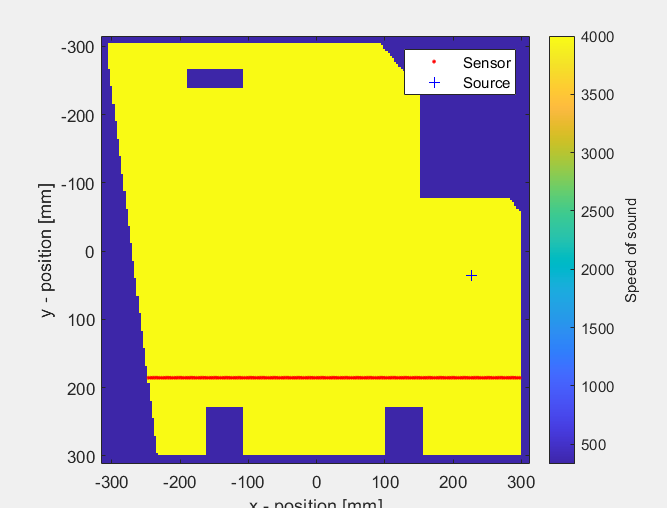
\includegraphics[width=.95\linewidth]{forme1.png}
    \caption{}
    \label{fig:sfig1}
  \end{subfigure}%
  \begin{subfigure}{.155\textwidth}
    \centering
    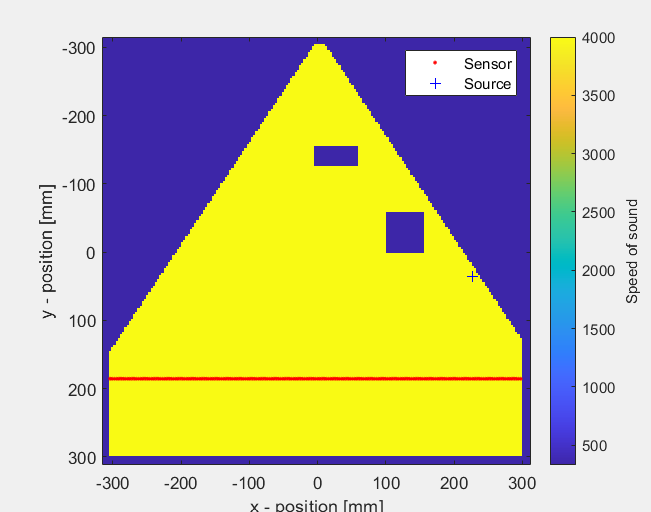
\includegraphics[width=.95\linewidth]{forme2.png}
    \caption{}
    \label{fig:sfig2}
  \end{subfigure}
  \begin{subfigure}{.155\textwidth}
    \centering
    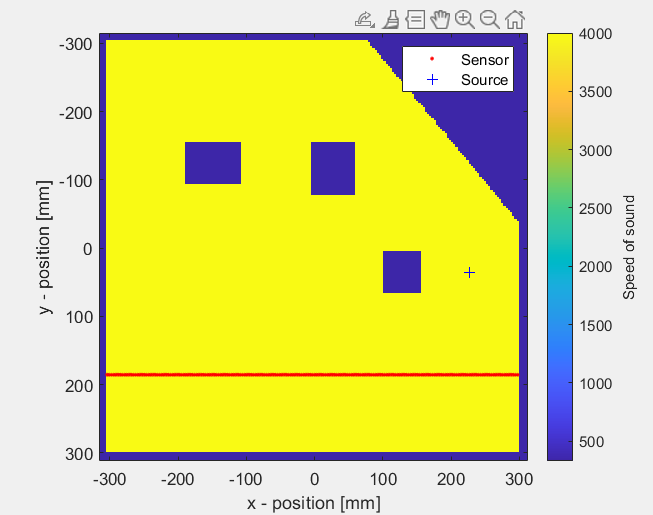
\includegraphics[width=.95\linewidth]{forme3.png}
    \caption{}
    \label{fig:sfig3}
  \end{subfigure}
  \begin{subfigure}{.155\textwidth}
    \centering
    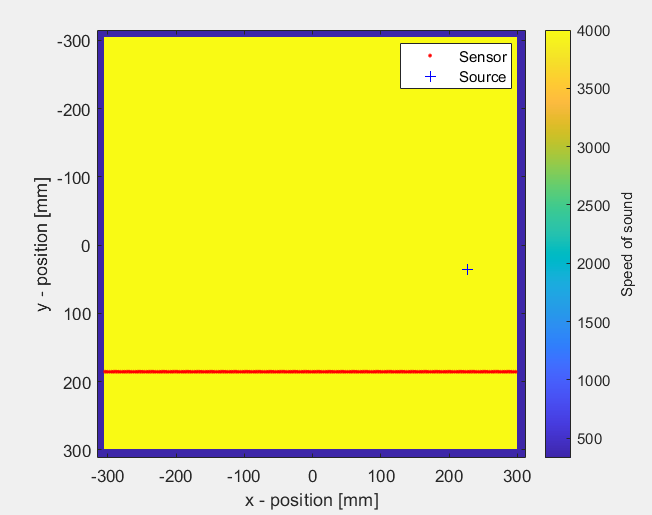
\includegraphics[width=.95\linewidth]{forme4.png}
    \caption{}
    \label{fig:sfig4}
  \end{subfigure}
  \begin{subfigure}{.155\textwidth}
    \centering
    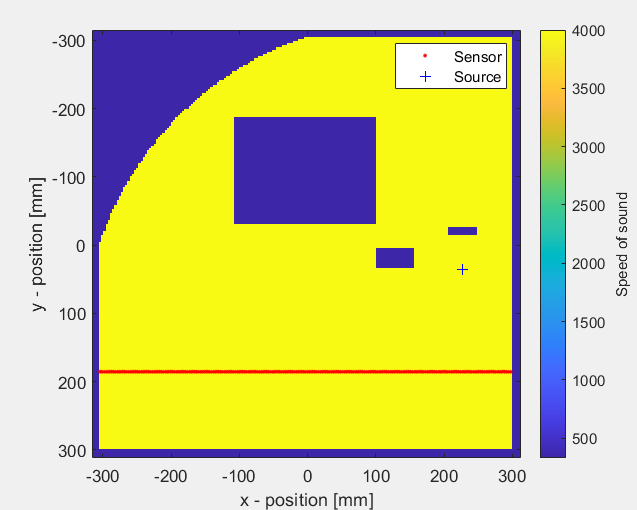
\includegraphics[width=.95\linewidth]{forme5.png}
    \caption{}
    \label{fig:sfig5}
  \end{subfigure}
  \begin{subfigure}{.155\textwidth}
    \centering
    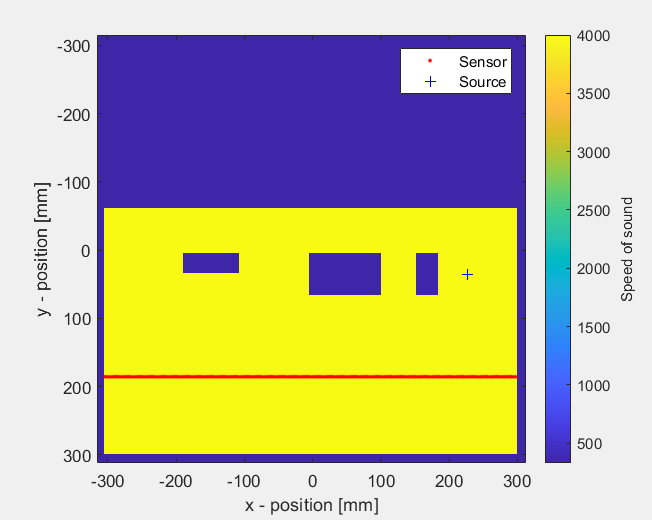
\includegraphics[width=.95\linewidth]{forme6.png}
    \caption{}
    \label{fig:sfig6}
  \end{subfigure}
  \caption{Géométries considérées pour les simulations}
  \label{fig:fig}
\end{figure}
Pour chaque géométrie, trois positions arbitraires pour le capteur ont été choisies,
chacune étant associée à un ensemble de coordonnées. À titre de référence, la position $(0,0)$ se situe 
en haut à gauche des grilles des figures \ref{fig:sfig1} à \ref{fig:sfig6}.  

\begin{table}[H]
\begin{tabularx}{\columnwidth}{@{} Y{1.00} Y{0.75} Y{1.00} Y{1.35} Y{0.87} @{}}
  \hline
  Matériau&Géométrie&Position du capteur&Contraste&Résolution\\
  \hline
  \multicolumn{5}{c}{Valeurs de contraste les plus élevées}\\
  \hline
  Plexiglas&(a)& 100, 100& $0.83 \pm 0.01$ & $8 \pm 1$ \\
  Plexiglas&(c)& 20, 100& $0.825 \pm 0.008$ & $7.7 \pm 0.2$ \\
  Plexiglas&(a)& 50, 100& $0.823 \pm 0.006$ & $8.4 \pm 0.8$ \\
  \hline
  \multicolumn{5}{c}{Valeurs de contraste les plus faibles}\\
  \hline
  Aluminium&(b)& 25, 100& $0.75 \pm 0.02$ & $15 \pm 2$ \\
  Aluminium&(e)& 110, 170& $0.76 \pm 0.01$ & $6.6 \pm 0.5$ \\
  Aluminium&(f)& 100, 30& $0.768 \pm 0.006$ & $12 \pm 2$ \\
  \hline
  \multicolumn{5}{c}{Valeurs de résolution les plus élevées}\\
  \hline
  Aluminium&(e)& 110, 100& $0.80 \pm 0.01$ & $15 \pm 2$ \\
  Aluminium&(b)& 25, 100& $0.75 \pm 0.02$ & $15 \pm 2$ \\
  Aluminium&(a)& 100, 100& $0.82 \pm 0.02$ & $15 \pm 4$ \\
  \hline
  \multicolumn{5}{c}{Valeurs de résolution les plus faibles}\\
  \hline
  Plexiglas&(e)& 30, 100& $0.803 \pm 0.006$ & $8 \pm 1$ \\
  Plexiglas&(c)& 20, 100& $0.825 \pm 0.008$ & $7.7 \pm 0.2$ \\
  Plexiglas&(a)& 50, 100& $0.823 \pm 0.006$ & $8.4 \pm 0.8$ \\
  \hline
\end{tabularx}
\caption{Résumé des résultats des simulations}
\label{tableau_resultats}
\end{table}
En guise de résumé, les cas ayant les valeurs de contraste et de résolution les plus faibles et les plus élevées
sont présentés dans le tableau \ref{tableau_resultats}. Les valeurs de contraste et de 
résolution correspondent chacune à la moyenne de l'ensemble de données, et leur incertitude 
correspond à l'écart-type.

%Spécifier que ces valeurs servent de référence pour les ordres de 
%grandeur mais PAS d'outil de décision ou que vaguement d'indicateur

%Ajouter des tableaux comparatifs en changeant un seul paramètre?


\section{Discussion}
% % Ayant obtenu un fit 2D gaussien, il est possible d'analyser et de comparer les variables
% % pertinentes, le contraste et la résolution, selon différents paramètres physiques qui 
% % ont été élaborés dans la section \ref{}. Le graphique \ref{} offre un échantillon des 
% % résultats obtenus pour une plaque carrée, sans trous et en bois. En ayant utilisé le 
% % retournement temporel, la durée de simulation a pu être réduite, ce qui a permis 
% % d'obtenir des réponses temporelles pour un nombre d'échantillons considérablement plus 
% % grand. Cette décision a permis d'améliorer la définition des fits gaussiens. Six 
% % échantillons ont été choisis au hasard parmi les deux bandes considérées, offrant un
% % poids statistique aux résultats assez important.

% % En observant le graphique \ref{}, on peut noter que l'emplacement de la source du signal
% % correspond à une corrélation de 1. Ceci s'explique facilement par le fait que le signal
% % choisi au hasard comme source et le signal de référence sont les mêmes (le choix de 
% % réutiliser le signal a été fait encore une fois pour réduire le temps de compilation). 
% % La courbe gaussienne a une correspondance quasi parfaite pour les données proches du 
% % maximum du pic, mais réduit en terme d'exactitude pour les données au niveau de la base
% % de la gaussienne.

% % En évaluant l'allure de la courbe pour le cas ci-présent, on peut 
% % estimer qu'il serait souhaitable de trouver des paramètres offrant un contraste plus 
% % grand que ceux évalués ici. La résolution, quant-à-elle, semble déjà suffisament bonne.
% % Évidemment, il est difficile d'arriver à une conclusion pertinente sans d'autres 
% % éléments de comparaison.

%1.  Explication de quels paramètres on prend: Énoncement du choix total, pourquoi? pour
%chaque choix, Méthode de choix (Choix des paramètres selon l'ordre du plus straight
%forward au moins), X
%2.  Incertitudes relatives (moins de 1%, important vu qu'on passe de simulé à réel, donc
%besoin d'une bonne confiance sur les valeurs obtenues) X
%3.  Limitations des simulations (pas de perte ni interférence par la table, trous carrés
%versus arrondis en vrai, etc.). Les simulations break down à densité et vitesse du 
%son élevées (i.e. brass & acier), donc on les a évité. (pas grave car plexi meilleur
%que Alu donc semble pas indiquer qu'on aurait de meilleurs résultats avec une plus 
%grande densité/vitesse du son). 
%D'ailleurs, ce n'est pas la seule situation qu'on a évité... 
%4.  Données aberrantes: Explication de leur provenance, choix d'éviter les 
%configurations qui les causent (matériaux et géométries), 

À la suite d'un plus grand nombre de simulations, les indicateurs de performance 
considérés pour le choix des paramètres sont une résolution fine, donc une 
préférence pour les valeurs de résolution les plus faibles, et un contraste 
important, donc une préférence pour les valeurs de contraste les plus grandes.
Avec ces considérations en tête, la configuration de la géométrie (c) en plexiglas 
avec le capteur en position (20,100) est celle retenue. Le choix de chaque paramètre
a été effectué en comparant sa performance à celle des configurations similaires, 
c'est-à-dire en ne changeant que ce paramètre tout en gardant les autres constants,
autant que possible.

Le premier paramètre à avoir été déterminé est le matériau. Pour ce paramètre, 
les performances de toutes les paires (géométrie, position du capteur) sont 
comparées. Mise à part lorsqu'il y a des données aberrantes, le plexiglas est 
meilleur que l'aluminium sur toutes les paires testées. Ce résultat systématique 
ne laisse aucune ambiguîté quant au choix à faire, donc c'est l'aluminium qui est 
choisi.

Le deuxième paramètre déterminé est la géométrie. Ce paramètre ne permet pas la 
comparaison par paires puisque la position du capteur est différente pour chaque 
géométrie. Il est considéré que la position du capteur est un degré de liberté 
dont on dispose lors que la fabrication du dispositif. Dans ce contexte, les
géométries sont comparées en fixant le matériau à du plexiglas, puisque ce choix
est déjà réalisé, et en prenant la meilleure résolution et le meilleur contraste
obtenus avec ce matériau. Les résultats obtenus pour ce paramètre sont mitigés, 
puisque les géométries (d) et (a) fournissent de les plus hauts contrastes mais des 
plus hautes résolutions, alors que les géométries (e) et (f) fournissent les plus 
hautes résolutions mais des plus bas contrastes. En observant les résultats en 
détail, on constate que le contraste varie entre 0,85 pour la meilleur géométrie 
et 0,80 pour la pire géométrie, alors que la résolution varie entre 6,0 mm pour la 
meilleure géométrie et 8,8 mm pour la pire géométrie. Même si la variation relative 
est plus grande pour la résolution, ces différences restent faible et même un duo 
de contraste de 0,8 et une résolution de 8,8 mm seraient satisfaisant. L'enjeu de la
faisabilité a également été pris en compte pour trancher la question pour ce 
paramètre. La géométrie (c) avec un capteur en (20,100) a donc été choisie 
puisqu'elle atteint la troisième place du contraste et de la résolution, avec un 
contraste de ($0,825 \pm 0,009$) et une résolution de ($7,7 \pm 0,2$)mm, tout en 
étant facile à réaliser. Les incertitudes relatives sur le contraste et la 
résolution sont d'environ respectivement 1\% et 3\%, ce qui est suffisament 
faible pour considérer les résultats significatifs. On peut avoir confiance que 
des valeurs d'ordre similaires seront obtenues lors de la réalisation concrète.

Le troisième paramètre, la position du capteur, est déterminé conjointement avec 
la géométrie, donc le choix de la position (20, 100) se doit d'être respecté. 

Il est important de mentionner que les simulations comportent plusieurs limitations.
La première de ces limitations est qu'il n'y a aucune interférence de la table ou 
du support dans les simulations, ce qui peut être un angle mort de l'étude présentée.
Comme il est probable que des pertes dans le signal soient occasionnées par ce
contact, il est décidé de tester l'identification de signal avec et sans matériel 
isolant le piano de son support. Une autre limitation a mentionner est que les trous
dans le matéériaux ne pourront pas être de forme carrée comme dans la simulation à 
cause de contrainte d'usinage. Il faut garder en tête l'arrondissement des coins dans
les causes potentielles d'erreurs lors de la fabrication et des tests du dispositif.
Enfin, il n'a pas été possible de simuler avec succès les matériaux dont la densité
est élevée. En effet, cette grande densité implique une vitesse du son trop élévée
pour la simulation. Lors des tests, l'onde sortait du matériau, ce qui est un résultat
non-physique dû au caractère discret des simulations. Cela implique qu'on n'a pas pu 
tester les métaux comme l'acier ou le laiton. Il a donc été décider de ne pas essayer
de faire un piano tactile avec ces matériaux, d'autant que la performance du plexiglas,
a surpasser celle de l'aluminium, laissant penser qu'une plus forte densité ne se 
traduit pas en une meilleure performance.

D'ailleurs, ce n'est pas la seule situation où les simulations ont montrées leurs 
limites. Il y a eu plusieurs données aberrantes: 
%Explication de leur provenance, choix d'éviter les 
%configurations qui les causent (matériaux et géométries),  

\clearpage

% \bibliographystyle{unsrtnat}
% \bibliography{My_Library}

\end{document}
